\section{Major themes}

\begin{marginfigure}
  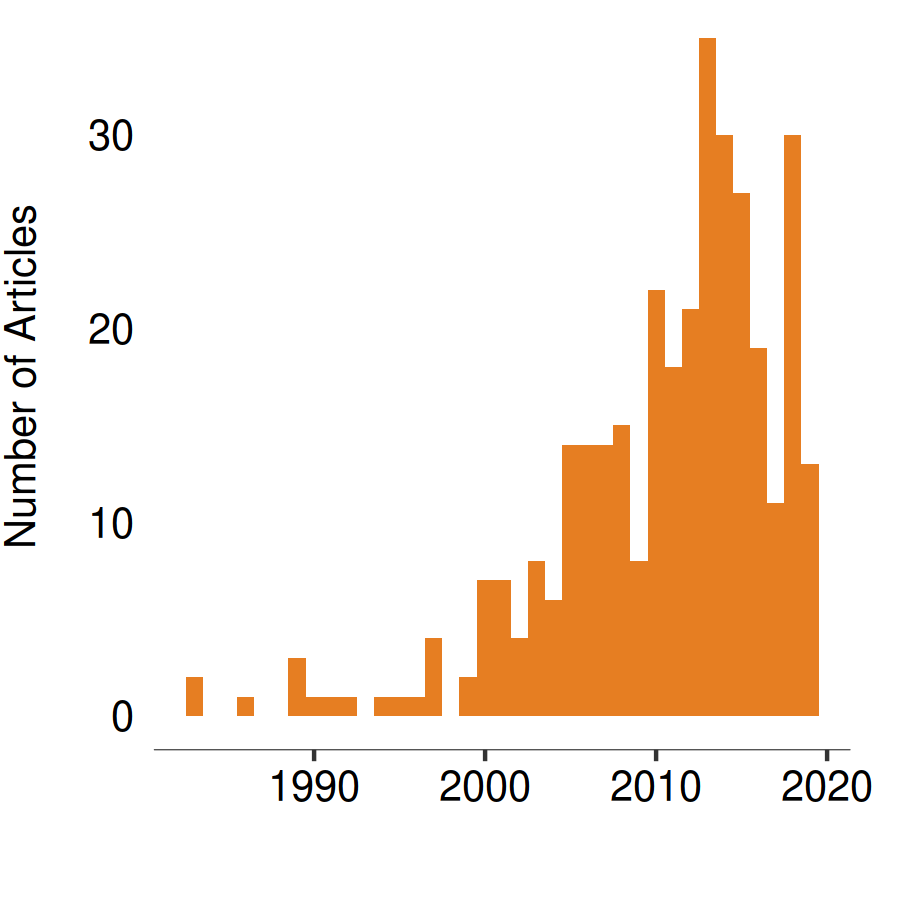
\includegraphics{images/literature-timeline.png}
  \caption{Growth of research in the topic of `'}
  \label{figure:literature:timeline}
\end{marginfigure}
\marginnote[1em]{\fontsize{7}{7}\textit{}}

There have been approximately 300 academic publications concerned with the high-resolution quantification of the spatio-temporal dynamics of urban movements.
It is clearly a multi-disciplinary topic that has been studied extensively under the fields of geography, urban studies, urban planning and management, emergency planning and management, economics, computer science and engineering, security and transportation planning.
Fig 1. shows the hierarchy themes as a tree map where the size shows the volume of research published.
We observe that the previous work can be classified into 5 major areas  - theory and methods, applications in studying mobility, applications in studying population, privacy and other areas which include de-anonymization, spatial classification, social networks and visualisation.

\begin{figure}
  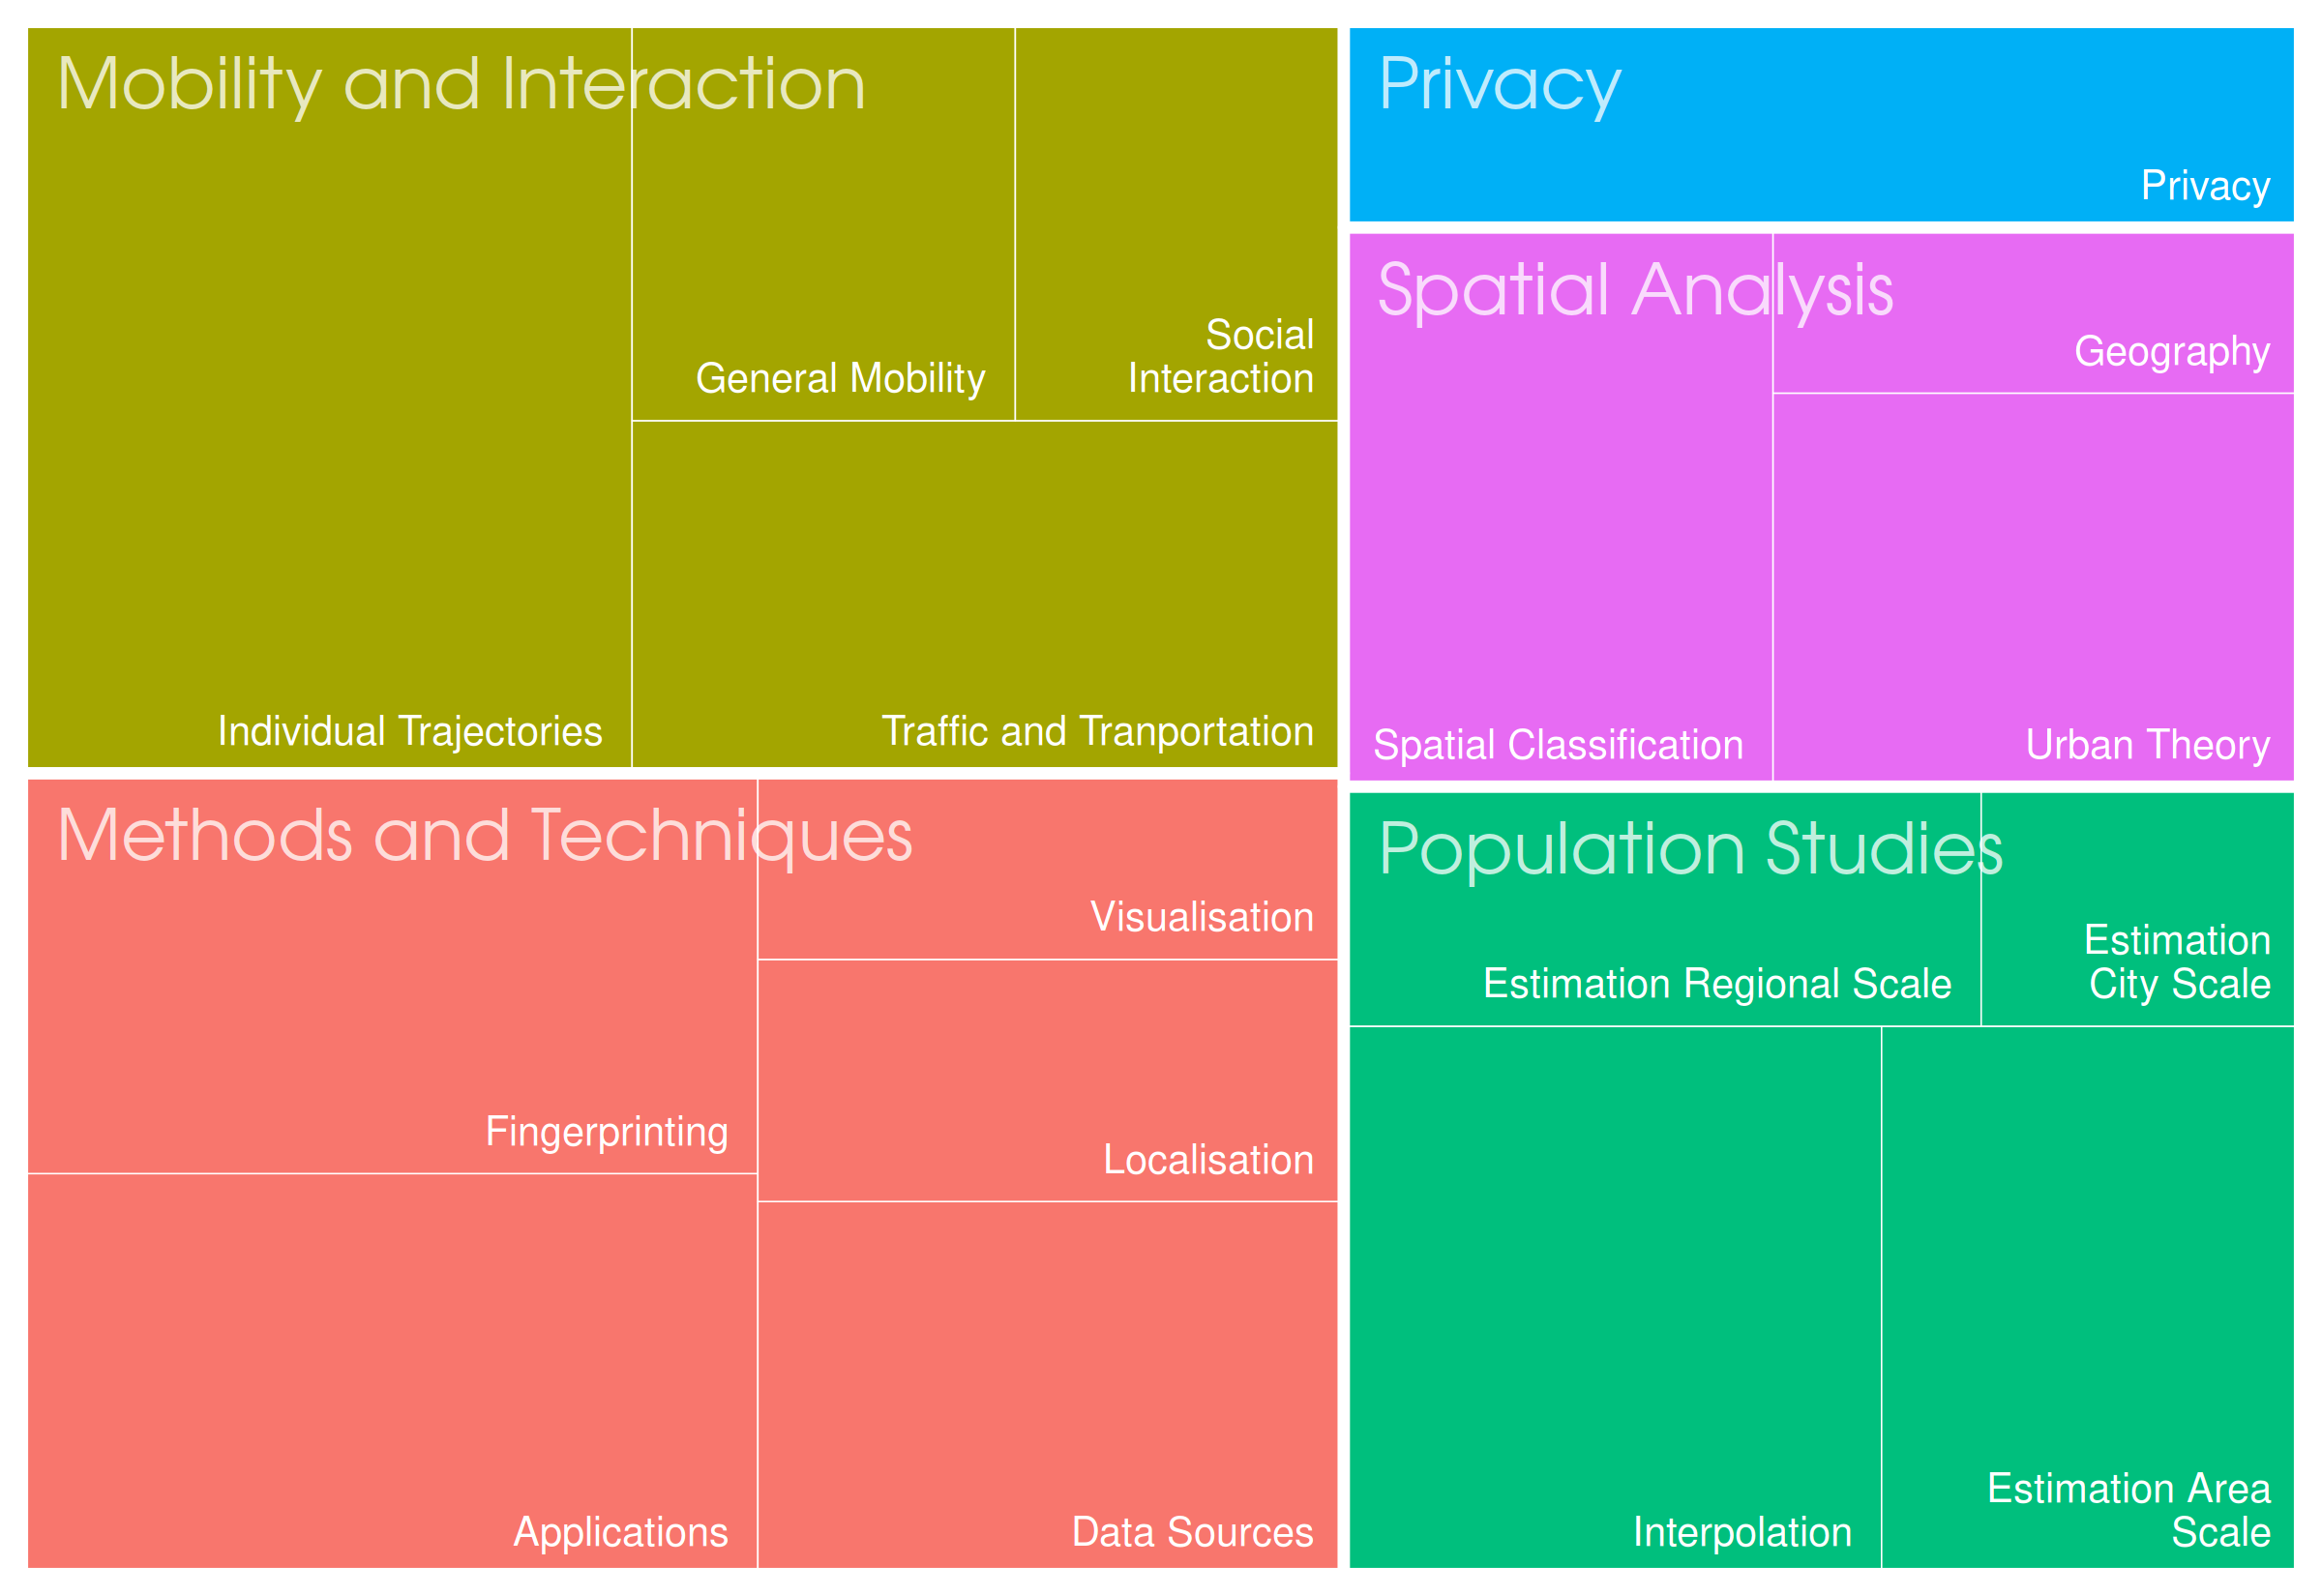
\includegraphics{images/literature-themes-treemap.png}
  \caption{Treemap showing the volume of research conducted under each major themes and their sub-themes.}
  \label{figure:literature:themes}
\end{figure}
\marginnote[-2.5in]{\textit{(Measured by the total number of articles or papers published)}}

\subsection{Population estimation and interpolation}
\subsection{Human Mobility and Interaction}
\subsection{Methodology and Techniques}
\subsection{Spatial Theory and Modelling}
\subsection{Privacy}

Traditional and modern geography were usually dominated by the study of centrally collected data acquired through extensive field surveys and remote sensing.
In the last two decades, a significant paradigm change has been introduced by the availability of unprecedented amount of data generated by unconventional sources such as mobile phones, social media posts etc.
This move to the postmodern geography (Soja, 1989) has been accompanied by a change in our understanding of the built environment and human geography, from a static point of view to a more dynamic definition based on the bottom up mechanisms which manifest in them, such as economic activity and information exchange (Batty 1990, 1997, 2012, 2013a,b).
This transition into the digital age (Graham, 1999; Tranos, 2012; 2013) has changed the politics of space and time (Massey, 1992) and been more pronounced in the study of urban built environment where technology has redefined the concepts of place and space (Graham, 2001; Sassen, 2001; Graham, 2002).
With the ability to collect and analyse of data on large complex systems in real-time (Graham, 1997), we are exploring the possibilities of understanding their structure and organisation using concepts of complexity theory (Bettencourt, 2013; Portugali, 2012) with more emphasis on their temporal patterns such as the argument towards finding the pulse of the city (Batty, 2010).
With the population getting more and more connected (Castells, 2010), the nature of space/place is being dynamically defined by the population themselves (Giuliano, 1991) and vice versa (Zandvliet, 2006).
This movement to the digital era was accompanied not only by optimism in its potential (Thomas, 2001; Nature, 2008) but also by the questions raised on the challenges in handling the diverse, large scale, non standardised data (Miller, 2010; Arribas-Bel, 2014 a) it produces and the usefulness or representativeness of the resulting analysis.
Nonetheless, availability of such data has impressive uses in urban studies (Bettencourt, 2014) especially with advancement of new technologies (Steenbruggen, 2015) and possibility of distributed, crowdsourced data collection (Lokanathan, 2015).
Visualising the temporal dynamics of data collected on human activities through decentralised processes poses significant challenges when approached with traditional cartographic concepts (MacEachren, 2001 Hallisey, 2005).
Digital media especially animation has been explored as an option to solve for the temporal dimension (Morrison, 2000; Lobben, 2003) but is bound by the cognitive limits of the viewer (Harrower, 2007).
There have been approaches proposed around animations of generated surfaces (Kobayashi, 2011) and network-based visualizations (Ferrara, 2014) leaving gaps in research for new methods in dynamic geo-visualisation (Fabrikant, 2005) and visualising path and flow of phenomena (Thomas, 2005).
This provides us with a promising opportunity for research in methods for visualising high frequency, hyper-local pedestrian data within the limits of cognition of the viewer.

As we can see from Figure 2. population studies and urban mobility are the most significant themes in this area of research.
Population studies include interpolation and estimation of population at small scales by using either traditionally available large-scale data (Sutton, 1997, Yuan, 1997) or newly available mobile device based data (Yuan, 2016) or a combination of both (Rao, 2015).
Urban mobility studies include collection and study of trajectories of mobile devices to understand human mobility at small scales and traffic and transportation studies at large scales.
Urban mobility research significantly benefited from the decentralised collection of granular data (Castells, 2000) and its augmentation through traditional models of travel behaviour (Janssens, 2013).
The large volume of research done under these themes is discussed in detail in the section on techniques and technologies.

The rise in personal technology has many opportunities for researchers and industry but at the same time has increased the general concern on privacy (Saponas, 2007; Krumm, 2009).
There is immense value in uniquely identifying and profiling information on people for specific purposes such as security (Cutter, 2006) and law enforcement (Dobson, 2003) but also has extreme risks associated when not handled with care (VanWey, 2005).
Strictly protecting personal information while ensuring the information is usable for research by maintaining the uniqueness in the data is the major concern which leads us to frameworks for secure practices in confidentially collecting and using the location data (Duckham, 2006; Tang, 2006; Lane, 2014).
Some efforts seek to accomplish this through cryptographic hashing algorithms (Pang, 2007) while others aim to thwart identification and tracking at the device level by techniques such as MAC randomisation (Gruteser, 2005; Greenstein, 2008).
The consent of users’ for the collection and use of such information from their mobile devices is low but with smart devices becoming ubiquitous there is a significantly improved acceptance when the process offers value in return such as discounts and monetary benefits (Kobsa, 2014) .

\subsection{Trends over time}

Figure 1 shows the volume of research done in this topic throughout years categorised based on their major themes discussed above.
We can observe that there are distinct trends in the research over time, with the explosion of interest in the last decade.
The research was mostly centered around population studies on interpolating larger datasets.
The period between 1990-2000 there was interest in potential of the new data generated by the digital age this coincided with mobile phones becoming more popular and ubiquitous with population in urban areas.
The next 5 years equal interest is observed in applying the data for population and urban mobility studies and in the development of theory, methods to use the data.
Between 2005 and 2010 the ‘mobile era’ saw significant rise in the volume of research, especially research focused on urban mobility and localisation and identification of the unique devices from the massive cellular network data which was met with an equal interest in privacy and data security.

\begin{figure*}
  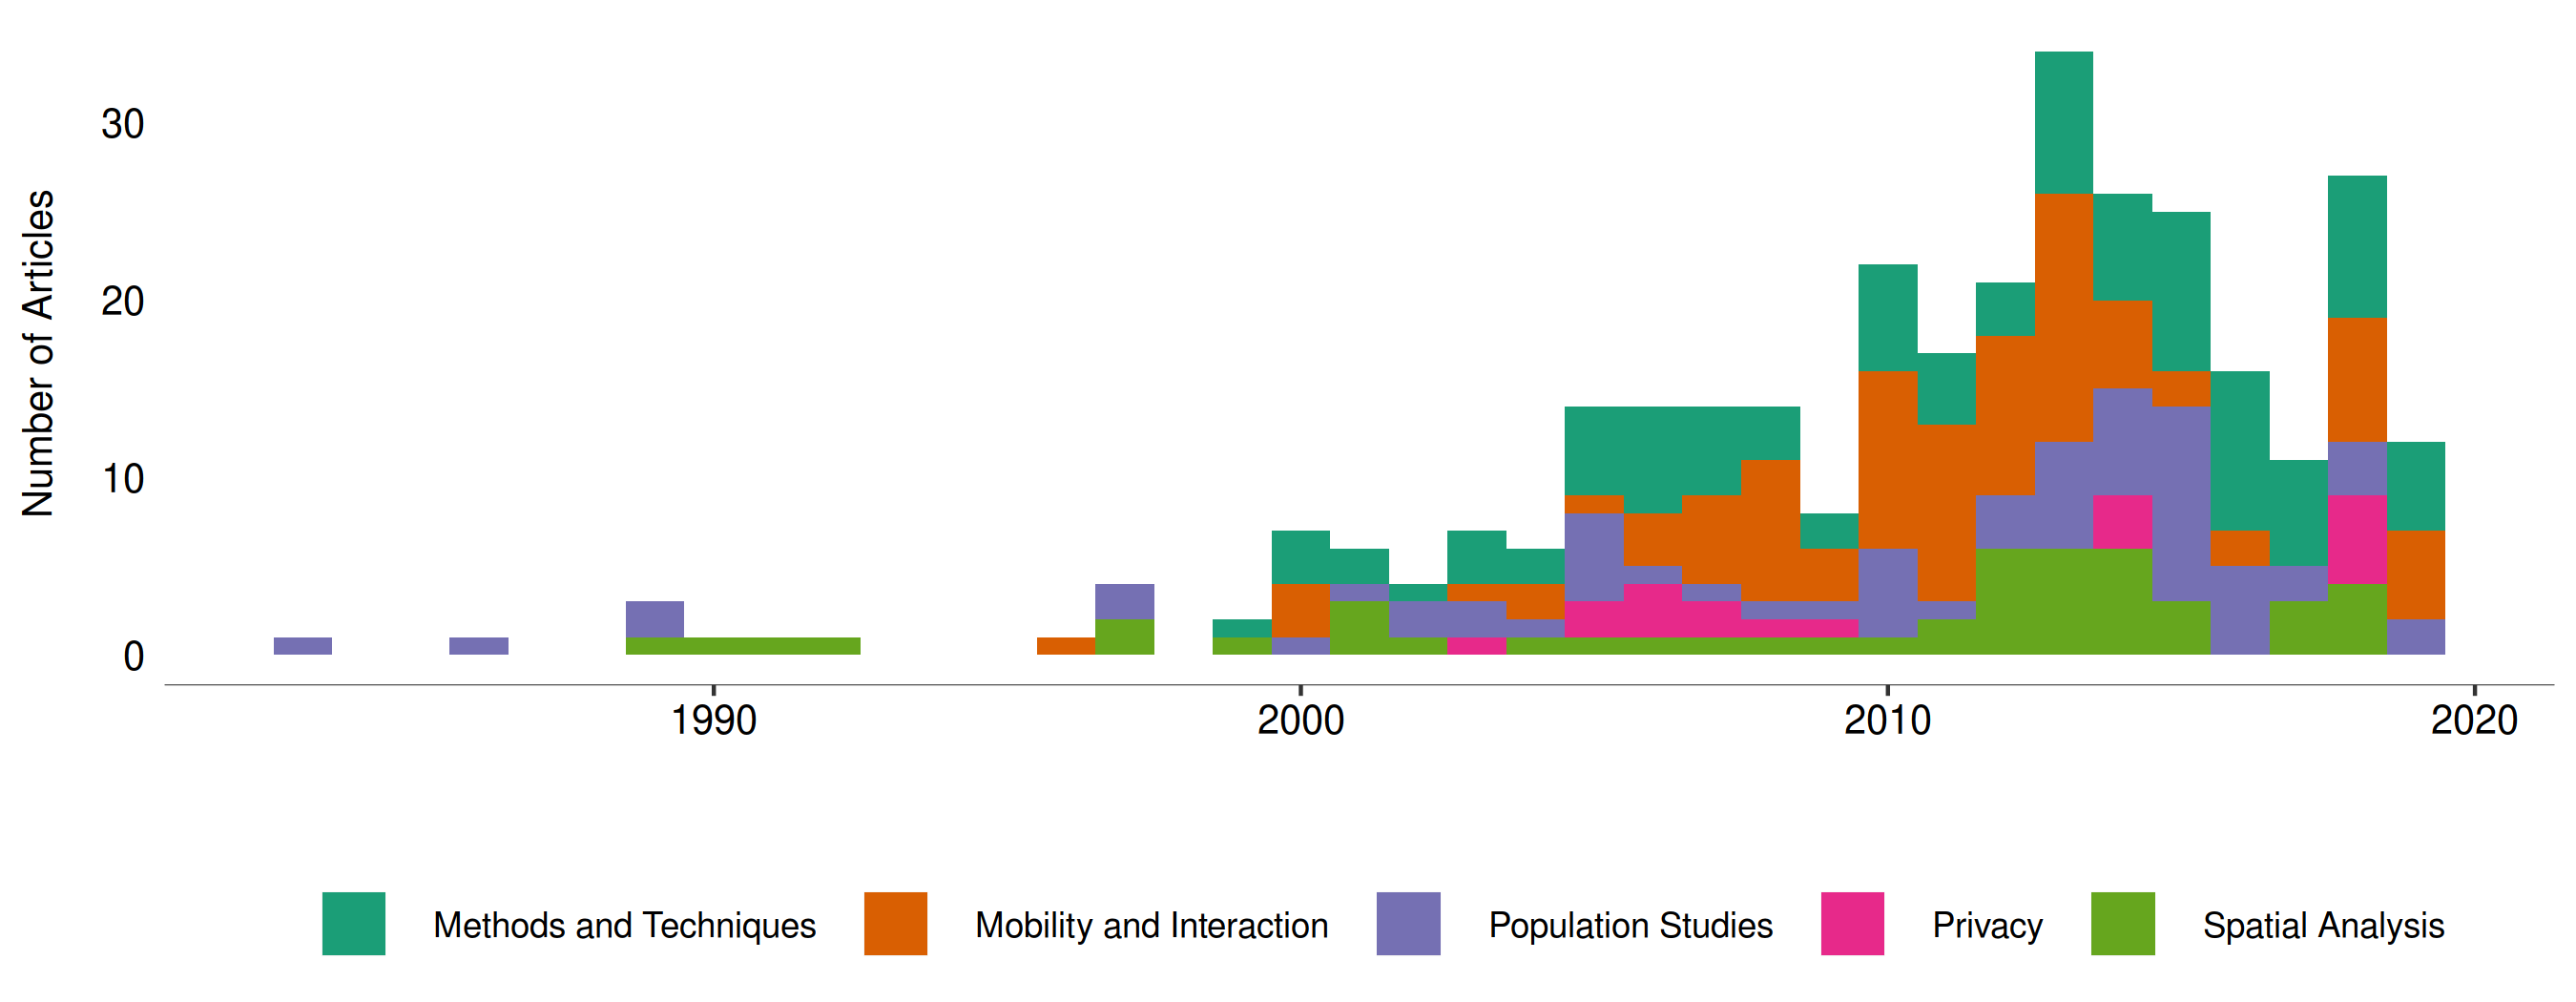
\includegraphics{images/literature-themes-timeline.png}
  \caption{Outline of the `Medium data toolkit' devised to collect, process, visualise and manage the Wi-Fi probe requests data}
  \label{figure:literature:themes:timeline}
\end{figure*}

In 2010 there was a clear increase in the volume of the research concerned with urban mobility, especially on tracking devices for trajectories.
This might be due to the emergence and proliferation of ‘smartphones’ around that time, which made collecting data from these devices directly much easier and less reliant on carrier provided datasets.
We also observe a focus on inferring the nature of the spaces these devices occupy and the social interactions between those who own these devices.
With the theoretical limit to predictability in human mobility quantified, the focus on urban mobility has been declining in the past few years.
This has been replaced by a renewed interest in population studies at a real-time, hyper-local level.
We also see a recent increase in interest in deanonymization in response to the industry adopting anti-tracking mechanisms in their products for example MAC randomisation in iOS devices.
Currently the research interest and gaps in the field concern the hyper-local estimation of population and nature along with methods to identify unique devices at this scale.
